\providecommand{\main}{../..}%define path to bib for subfiles
\documentclass[../../main.tex]{subfiles}
\begin{document}
\onlyinsubfile{\setcounter{chapter}{8}}
\notinsubfile{}
\subsection*{Shor's algoritme kraakt RSA encryptie}
Het RSA encryptie-protocol is een van de twee standaard versleutelmethoden waarmee we beveiligde berichten versturen (zoals bijvoorbeeld banktransacties). \marginpar{\footnotesize{De andere is Diffie-Hellman, en die kan ook met quantumcomputing gekraakt worden.}}
Het is gebaseerd op een asymmetrisch probleem: het is eenvoudig om het product van twee grote priemgetallen uit te rekenen, maar het is heel moeilijk om in een groot getal twee priemfactoren terug te vinden. Het getal $N$ dat RSA hiervoor gebruikt is in de loop der tijd steeds groter geworden. Tegenwoordig wordt een getal van $N=2048$ cijfers of meer ($N=4096$) gebruikt. Het getal zelf is dus onuitspreekbaar groot.\marginpar{\footnotesize{Als $N=6$, dan is het getal zelf $10^6$: in de orde van een miljoen. $N$ geeft de log van het getal weer.}}

\marginpar{een product reken je makkelijk uit:\\101*103=10403, maar wat zijn de factoren van 78373?} %31*37=1147%181*433=78373
\begin{antwoord}[3.5cm]
181*433=78373
\end{antwoord}

We moeten hier een diepere beschrijving van RSA achterwege laten, maar zullen proberen te schetsen waar quantumcomputing de achilleshiel in RSA vindt. Zowel in de encryptie als in het kraken van RSA staat een stelling uit de getaltheorie centraal:  Als je een willekeurig getal $a$, dat geen factor is van $N$ (anders ben je al klaar), telkens maar met zichzelf vermenigvuldigt ($a^k$) en je deelt het door $N$ dan vertoont de rest van de deling ($t$) een herhalend gedrag. De periode van deze herhaling geeft op zijn beurt een aanwijzing voor de factoren van $N$. Als je daar meer over wilt weten zie \cite{Aaronson2007,Wolf2021}. Een voorbeeldje (zie figuur~\ref{fig:shorrest})

\marginpar{\footnotesize{ $ x = a^k \pmod N$ }}

\begin{flushleft}
\begin{minipage}{.55\textwidth}
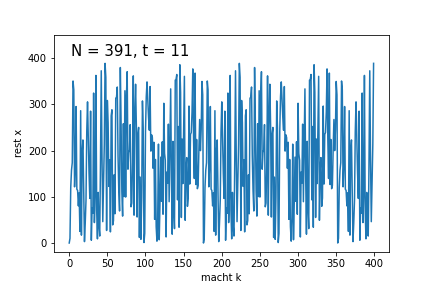
\includegraphics[width=\textwidth]{./img/shor_N=391_t=11.png}
\end{minipage}%
\hfill
\begin{minipage}{.4\textwidth}
\captionof{figure}{De functie $ x = a^k \pmod N$ ziet er grillig uit. Kun je de herhalingsperiode vinden?\label{fig:shorrest}}
\end{minipage}%
\end{flushleft}
\begin{antwoord}[-4cm]
176
\end{antwoord}
Maar de stelling heeft het er niet over dat dit een gigantische hoeveelheid rekenwerk kan kosten. De rekentijd die nodig is om een getal te ontbinden neemt exponentieel toe met de grootte van dat getal $O(2^{\log N})$. Voor grote getallen is dit onbegonnen werk. Toch zit de clou in die periodiciteit. 
\marginpar{Teken op je grafische rekenmachine de functies $y=2^x$, $y=x$,  $y=x^2$ en $y=x^3$.}

Er is een wiskundige operatie Fouriertransformatie, waarmee je \textit{zonder informatieverlies} periodiciteit in een signaal kunt vinden. Meestal van tijd naar frequentie of van afstand naar dichtheid (1/afstand). Zo zijn in het experiment van hoofdstuk~\ref{chap:H1} de patronen op de muur en in het kaartje bij ons spletenexperiment elkaars Fourier-getransformeerde. De transformatie kan zowel heen als terug zonder verlies van informatie, wat natuurlijk een voorwaarde is voor een quantumversie van de transformatie (waarom?). Het volgende voorbeeld laat de kracht van de techniek zien. 


\textbf{periodiciteit} Stel je bent proefpersoon in een experiment waarin je bioritme wordt bepaald. In het experiment verblijf je een paar dagen in een kamer zonder ramen, en zonder contact met de buitenwereld. Je wordt uit jezelf wakker en je gaat uit jezelf naar bed als je moe bent. In de kamer hangen een aantal 24-uurs klokken met alleen een uurwijzer. Onder de klokken hangt een papiertje. Telkens als je wakker wordt teken je hier de wijzer in de richting waarin deze dan staat in het  verlengde van waar je de vorige dag ge\"eindigd bent. De klokken lopen allemaal in een verschillend tempo, te snel of te langzaam, maar eentje komt overeen met jouw bioritme. Als de klok veel te snel of veel te langzaam loopt, komen na een paar dagen de streepjes in allerlei richtingen te staan en blijven ze op het papiertje.
Maar op het papiertje onder de klok die gelijk loopt met jouw bioritme komt het streepje telkens in dezelfde richting te staan. Je bent al gauw van het papier af. De gezochte oplossing wordt versterkt (constructieve interferentie) en  ongewenste oplossingen worden uitgedempt (destructieve interferentie).

\newcommand\klok[3][1.5]{%
\begin{tikzpicture}[scale=#1,line cap=round,line width=#1*3pt]
\filldraw [fill=yellow!20] (0,0) circle (2cm);
%\foreach \angle / \label in
%{0/6, 30/4, 60/2, 90/24, 120/22, 150/20, 180/18,
%210/16, 240/14, 270/12, 300/10, 330/8}
%{
%\draw[line width=#1*1pt] (\angle:1.8cm) -- (\angle:2cm);
%\draw (\angle:1.4cm) node[scale=#1]{\textsf{\label}};
%}
%\foreach \angle in {0,90,180,270}
%\draw[line width=#1*2pt] (\angle:1.6cm) -- (\angle:2cm);
\node[draw=none,scale=#1*2] at (0,.9cm) {#3};
\draw[rotate=90,line width=#1*2pt] (0,0) -- (-#2*15:0.7cm); % hours
\path [fill=black] (0,0) circle (3pt);
\path [fill=red] (0,0) circle (1.5pt);
%
\draw [fill=yellow,yellow] (-1cm,-4.5cm) rectangle (1cm,-2.5cm); 
\end{tikzpicture}%
}
%%\syntax
%% \clock[<optional scaling dim>]{<hour>}{tekst}

\klok[.3]{7}{traag}\hfill\klok[.3]{8}{normaal}\hfill\klok[.3]{9}{snel}

\nogdoen{Met een beetje fantasie zie je in de klokken de qubits terug die ronddraaien op de eenheidscirkel. Ze zijn geprogrammeerd om op hun eigen frequentie te draaien.}Peter Shor zag in dat de quantumversie van Fouriertransformatie de sleutel is tot het kraken van RSA. De langzaamste stap van het algoritme wordt overgenomen door een quantumcomputer. De tijd die nodig is om een getal te ontbinden wordt van exponentieel $O(2^{\log N})$ teruggebracht tot ($O(\log\log N)$. Een quntumcomputer heeft iests meer dan 4096 perfecte qubits nodog om RSA-2048 te kraken. Het is een kwestie van wachten tot quantumcomputers sterk genoeg zijn deze klus te klaren. Kijk naar een \hrefqr{https://www.youtube.com/watch?v=hOlOY7NyMfs&ab_channel=PhysicsWorld}{korte uitleg} van Peter Shor zelf.

Nu is encryptie een wapenwedloop tussen versleutelaars en krakers. Met RSA stonden de versleutelaars heel lang voor. De gevolgen van Shor's algoritme zijn groot. Informatie die (sinds decennia) versleuteld on-line is komen te staan zal dan een open boek zijn. Gelukkig is de volgende stap in de wapenwedloop weer gezet: post quantum encryptie. Een eenvoudig voorbeeld van quantum versleuteling vind je in praktische opdracht~\ref{sec:poBB84}.
\end{document}
